%%%%%%%%%%%%%%%%%%%%%%%%%%%%%%%%%%%%%%%%%
% Beamer Presentation
% LaTeX Template
% Version 1.0 (10/11/12)
%
% This template has been downloaded from:
% http://www.LaTeXTemplates.com
%
% License:
% CC BY-NC-SA 3.0 (http://creativecommons.org/licenses/by-nc-sa/3.0/)
%
%%%%%%%%%%%%%%%%%%%%%%%%%%%%%%%%%%%%%%%%%

%----------------------------------------------------------------------------------------
%	PACKAGES AND THEMES
%----------------------------------------------------------------------------------------

\documentclass{beamer}
\usepackage[T1]{fontenc}
\usepackage{polski}
\usepackage[utf8]{inputenc}
\usepackage[polish]{babel}

\mode<presentation> {

% The Beamer class comes with a number of default slide themes
% which change the colors and layouts of slides. Below this is a list
% of all the themes, uncomment each in turn to see what they look like.

%\usetheme{default}
%\usetheme{AnnArbor}
%\usetheme{Antibes}
%\usetheme{Bergen}
%\usetheme{Berkeley}
%\usetheme{Berlin}
%\usetheme{Boadilla}
\usetheme{CambridgeUS}
%\usetheme{Copenhagen}
%\usetheme{Darmstadt}
%\usetheme{Dresden}
%\usetheme{Frankfurt}
%\usetheme{Goettingen}
%\usetheme{Hannover}
%\usetheme{Ilmenau}
%\usetheme{JuanLesPins}
%\usetheme{Luebeck}
%\usetheme{Madrid}
%\usetheme{Malmoe}
%\usetheme{Marburg}
%\usetheme{Montpellier}
%\usetheme{PaloAlto}
%\usetheme{Pittsburgh}
%\usetheme{Rochester}
%\usetheme{Singapore}
%\usetheme{Szeged}
%\usetheme{Warsaw}

% As well as themes, the Beamer class has a number of color themes
% for any slide theme. Uncomment each of these in turn to see how it
% changes the colors of your current slide theme.

%\usecolortheme{albatross}
%\usecolortheme{beaver}
%\usecolortheme{beetle}
%\usecolortheme{crane}
%\usecolortheme{dolphin}
%\usecolortheme{dove}
%\usecolortheme{fly}
%\usecolortheme{lily}
%\usecolortheme{orchid}
%\usecolortheme{rose}
%\usecolortheme{seagull}
%\usecolortheme{seahorse}
%\usecolortheme{whale}
%\usecolortheme{wolverine}

%\setbeamertemplate{footline} % To remove the footer line in all slides uncomment this line
%\setbeamertemplate{footline}[page number] % To replace the footer line in all slides with a simple slide count uncomment this line

%\setbeamertemplate{navigation symbols}{} % To remove the navigation symbols from the bottom of all slides uncomment this line
}

\usepackage{graphicx} % Allows including images
\usepackage{animate}
\usepackage{movie15}
\usepackage{subfig}
\usepackage{booktabs} % Allows the use of \toprule, \midrule and \bottomrule in tables
\usepackage[skip=2pt,font=scriptsize]{caption}
\usepackage{color}


%----------------------------------------------------------------------------------------
%	TITLE PAGE
%----------------------------------------------------------------------------------------

%\title[VIM]{Zwiększ swoją produktywność\\ ...czyli wybierz (naj)lepszy edytor} % The short title appears at the bottom of every slide, the full title is only on the title page
\title[VIM]{Wybierz najlepszy edytor\\i~dlaczego jest to VIM} % The short title appears at the bottom of every slide, the full title is only on the title page

\author{Karol Katerżawa} % Your name
\institute[IAiIS] % Your institution as it will appear on the bottom of every slide, may be shorthand to save space
{
Instytut Automatyki i~Informatyki Stosowanej \\ % Your institution for the title page
\medskip
\textit{\textbf{Promotor:} dr~inż. Tomasz Kornuta} % Your email address
}
\date{\today} % Date, can be changed to a custom date
%\date{21.02.2014 r.} % Data obrony

%----------------------------------------------------------------------------------
% FRAME NUMBERING MACRO
%----------------------------------------------------------------------------------
%\expandafter\def\expandafter\insertshorttitle\expandafter{%
%  \insertshorttitle\hfill%
%  \insertframenumber\,/\,\inserttotalframenumber}
%  
%\setbeamerfont{caption name}{size=\tiny}
%\setlength{\textfloatsep}{5pt plus 1.0pt minus 2.0pt}
%\setlength{\floatsep}{5pt plus 1.0pt minus 2.0pt}
%---------------------------------------------------------------------------------------
% BEGIN DOCUMENT
%---------------------------------------------------------------------------------------
\begin{document}

\begin{frame}
\titlepage % Print the title page as the first slide
\end{frame}

%\begin{frame}
%\frametitle{Overview} % Table of contents slide, comment this block out to remove it
%\tableofcontents % Throughout your presentation, if you choose to use \section{} and \subsection{} commands, these will automatically be printed on this slide as an overview of your presentation
%\end{frame}

%----------------------------------------------------------------------------------------
%	PRESENTATION SLIDES
%----------------------------------------------------------------------------------------

\section{Wprowadzenie}
\label{sec:Wprowadzenie}

\begin{frame}[t]{Jaki edytor wybrać?}
  \begin{block}{Kryteria wyboru}
    \begin{itemize}
      \item Przeznaczenie
      \item Łatwość obsługi
      \item Możliwości
      \item Estetyka
      \item Szybkość działania
      \item Przenośność
      \item Cena
    \end{itemize}
  \end{block}
\end{frame}

\begin{frame}[t]{Typy edytorów}
  \begin{itemize}
    \item zwykły notatnik (np. notatnik, gedit)
    \item lepszy notatnik (np. Notepad++, geany, TextMate, Sublime Text)
    \item IDE (np. Eclipse, IntelliJ IDEA, Netbeans)
  \end{itemize}
%\begin{figure}[!h]
% \centering
% \subfloat[\tiny Subfigure caption]{\includegraphics[width=0.45\textwidth, clip]{image_1}}
% \subfloat[\tiny Subfigure caption]{\includegraphics[width=0.45\textwidth, clip]{image_2}}
% \setbeamerfont{caption name}{size=\tiny}
% %\vspace{-10pt}
% \caption{\tiny Figure caption}
%\end{figure}
\end{frame}

\begin{frame}[t]{VIM - edytor hakera?}
%\begin{figure}
%\centering
%\includegraphics[width=0.8\textwidth]{images/matrix.gif}
%\includemovie{5cm}{5cm}{images/matrix.gif}
%\end{figure}
  \animategraphics[width=0.8\textwidth,autoplay,controls]{12}{images/imgpdf/matrix_}{0}{10}
\end{frame}

\section{Przewaga VIMa}
\label{sec:Przewaga VIMa}

\begin{frame}[t]{VIM - edytor hakera?}
%\begin{figure}
%\centering
%\includegraphics[width=0.8\textwidth]{images/matrix.gif}
%\includemovie{5cm}{5cm}{images/matrix.gif}
%\end{figure}
\end{frame}

\begin{frame}[t]{Ergonomia, szybkość i~wygoda}
\begin{figure}
\centering
\vspace{-15pt}
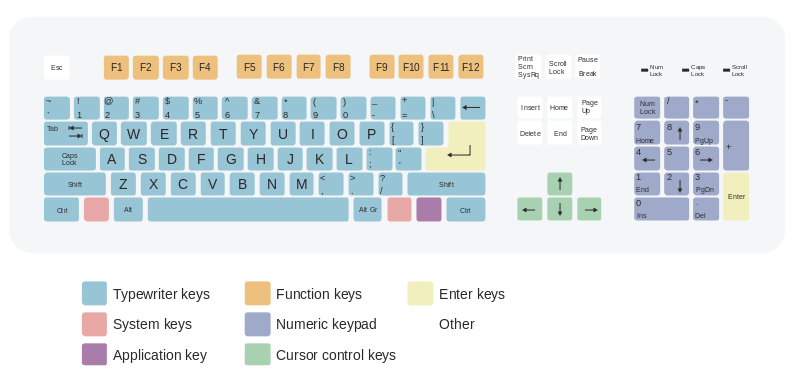
\includegraphics[width=0.8\textwidth]{images/full_keyboard}
\end{figure}
\begin{figure}
\centering
\vspace{-10pt}
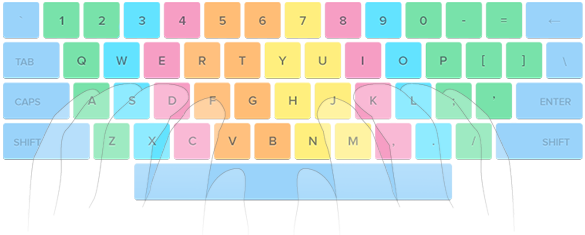
\includegraphics[width=0.6\textwidth]{images/edu_keyboard}
\end{figure}
\end{frame}

\begin{frame}[t]{Powtarzalność}
  \begin{itemize}
    \item Powtórzenie ostatniej komendy
    \item Wielokrotne wykonanie tej samej komendy
    \item Makra i~wiele innych
  \end{itemize}
\end{frame}

\begin{frame}[t]{Edytor modalny}
  \begin{block}{Tryby podstawowe}
    \begin{itemize}
      \item normal
      \item insert
      \item visual
      \item replace
      \item command
    \end{itemize}
  \end{block}
\end{frame}

\section{Jak się nauczyć?}
\label{sec:Jak się nauczyć?}

\begin{frame}[t]{Naucz się komend}
%  \begin{figure}
%  \centering
%  \includegraphics[width=0.8\textwidth]{cheatsheets/all.gif}
%  \end{figure}
\end{frame}


\section{Droga VIMa}
\label{sec:Droga VIMa}


\section{First section}
\subsection{First subsection}
\begin{frame}
\frametitle{First frame}
\begin{block}{Block 1}
Content
\end{block}
\end{frame}

\subsection{Second subsection}
\begin{frame}
Some content
\end{frame}

%-----------------------------------------------------------------------------------------
\section{Rozpoznawanie obiektów w obrazach RGB-D}

\subsection{Schemat działania podsystemu}

\begin{frame}
\frametitle{Frame title}
\setbeamerfont{block body}{size=\tiny}
\fboxsep=0pt
\noindent{%
\begin{minipage}[t]{0.48\linewidth}
\begin{block}{Block 2}
\begin{itemize}
\item first item
\item second item
\item third item
\end{itemize}
\end{block} 
\end{minipage}}
\hfill

\begin{minipage}[t]{0.48\linewidth}
\begin{block}{Block 3}
\begin{enumerate}
\item first item
\item second item
\item third item
\end{enumerate}
\end{block}
%\begin{figure}
%\centering
%\includegraphics[width=0.8\textwidth]{image}
%\caption{\tiny caption}
%\end{figure}
\end{minipage}


\end{frame}



%-----------------------------------------------------------------------------------------
\section{Final section}

\subsection{Summary}
\begin{frame}
\frametitle{Summary}
\centerline{Thank you!}
\end{frame}

%\begin{figure}[!h]
%	\centering
%	\subfloat[\tiny Subfigure caption]{\includegraphics[width=0.45\textwidth, clip]{image_1}}
%	\subfloat[\tiny Subfigure caption]{\includegraphics[width=0.45\textwidth, clip]{image_2}}
%	\setbeamerfont{caption name}{size=\tiny}
%	%\vspace{-10pt}
%	\caption{\tiny Figure caption}
%\end{figure}


\end{document} 
